\documentclass[11pt]{article}
\usepackage[UTF8]{ctex}
\usepackage{graphicx}
\usepackage{geometry}
\usepackage{hyperref}
\usepackage{listings}
\usepackage{xcolor}
\usepackage{float}
\geometry{a4paper, margin=2.5cm}

\hypersetup{colorlinks=true, linkcolor=blue, urlcolor=blue}

\lstset{
  basicstyle=\ttfamily\small,
  breaklines=true,
  frame=single,
  backgroundcolor=\color{gray!10},
  columns=fullflexible,
}

\title{Lab0: GitLab 实验报告}
\author{李长川 \quad 25800180107}
\date{\today}

\begin{document}
\maketitle

\section{任务 1：问题回答}

\textbf{Q1. 你之前有过多人协同开发的经历吗？如果有，你们是使用什么方式分工协作的？}

\par 有过。课程作业和竞赛集训里和同学一起写过小程序。那时候靠微信群分工，代码互相发文件或者丢网盘，文件名经常变成 \texttt{main\_new.cpp}、\texttt{final\_final.cpp} 这种。合并时手动对比两份代码，改错了想回退只能重新要旧版本，也不知道是谁在什么时候改了哪一行。这次 Lab0 算是第一次正经用上版本控制。

\textbf{Q2. Git 为什么要设计"暂存--提交"两个步骤？}

\par 主要是为了让一次提交在语义上完整。工作区里经常同时堆着好几件不相关的改动，有了暂存区就可以只把属于同一逻辑的改动 \texttt{git add} 进去，再写一句准确的 commit message。提交前还能用 \texttt{git status} / \texttt{git diff --cached} 检查，加错了文件可以 \texttt{git restore --staged} 撤回来。另外用 \texttt{git add -p} 可以把同一文件里的不同 hunk 拆开分别提交，历史会干净很多。

\textbf{Q3. \texttt{git branch} 和 \texttt{git branch -a} 的区别是什么？}

\par \texttt{git branch} 只列出本地分支；\texttt{git branch -a}（--all）会同时列出远程跟踪分支，即 \texttt{remotes/origin/...} 那些。后者显示的远程分支是上一次 \texttt{git fetch} / \texttt{git pull} 时的快照，不是实时的；如果远程删了某个分支，本地还要 \texttt{git fetch --prune} 清理一下过期的远程跟踪分支。

\section{任务 2：模板建仓与 main.c}

\par 在课程给出的模板仓库 \texttt{ICS-26Fall-FDU/GitLab} 上点 \texttt{Use this template}，创建个人仓库 \texttt{ChangchuanLi25800180107}，然后在 WSL 里 \texttt{git clone} 到本地。

\par 打开 \texttt{main.c}，把 TODO 那一行的 \texttt{printf} 改成 \texttt{printf("What can I say\textbackslash n");}，保存后 \texttt{git add} / \texttt{git commit -m "Update main.c"} / \texttt{git push}。

\begin{figure}[H]
  \centering
  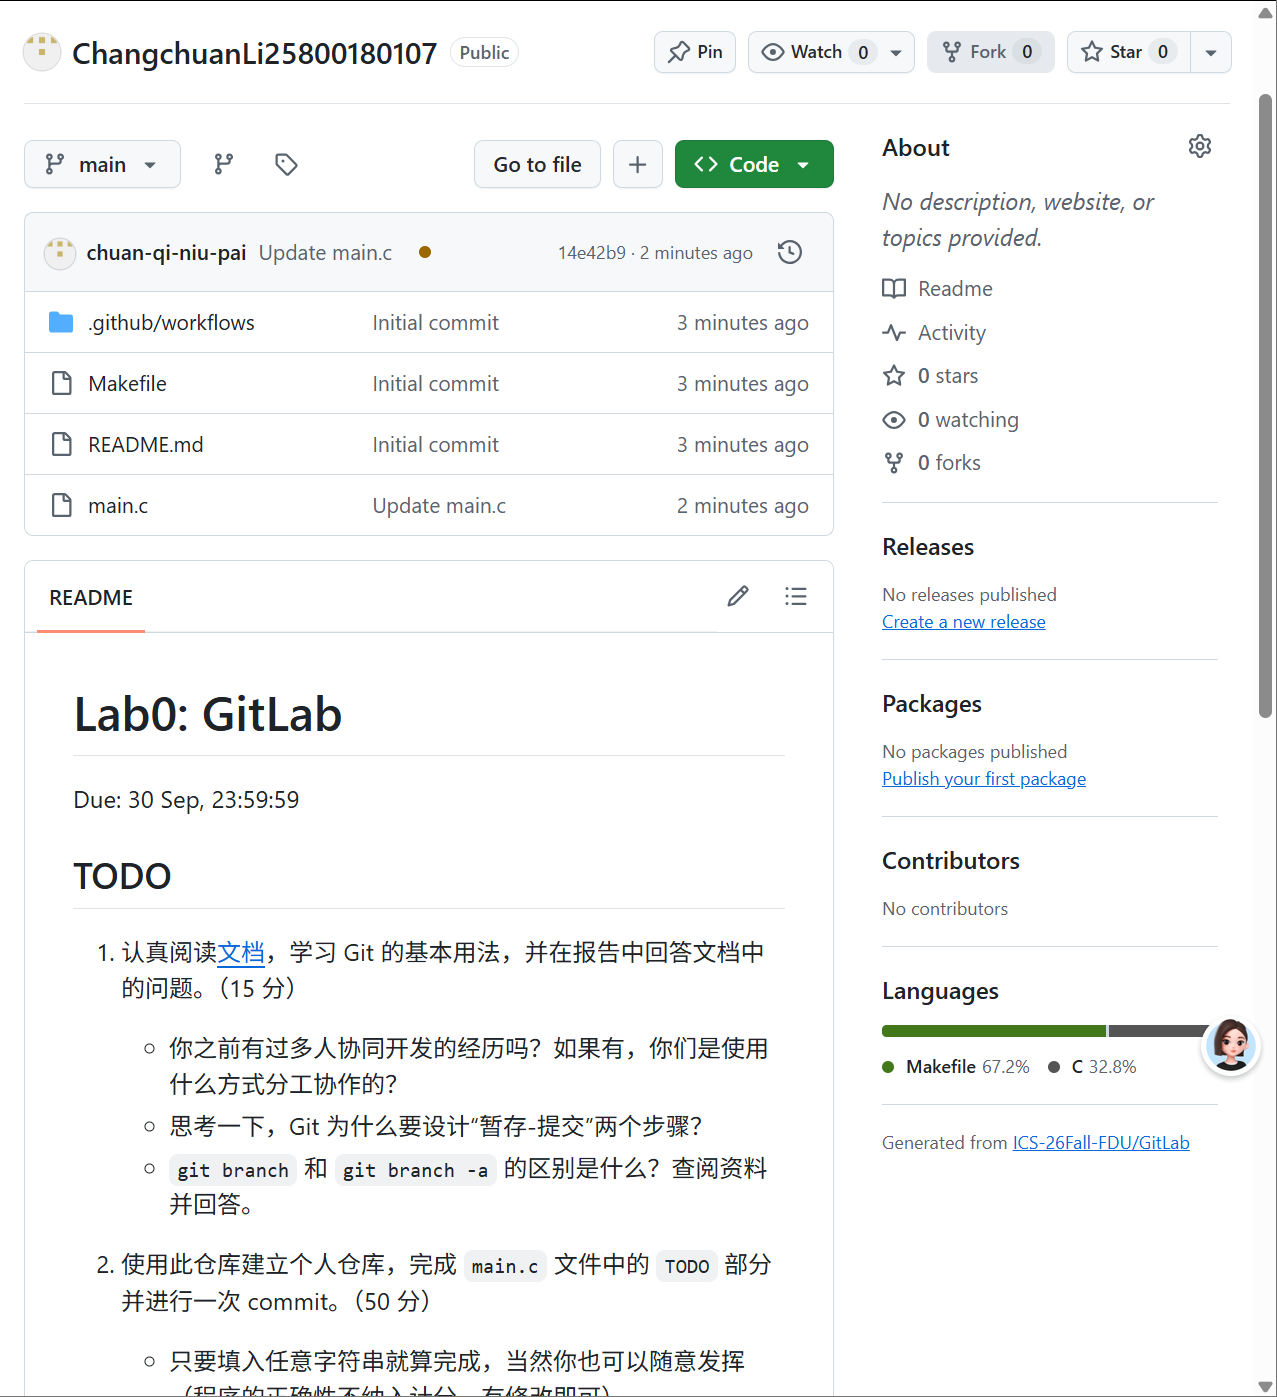
\includegraphics[width=0.85\textwidth]{images/repo_homepage.png}
  \caption{个人仓库主页}
\end{figure}

\begin{figure}[H]
  \centering
  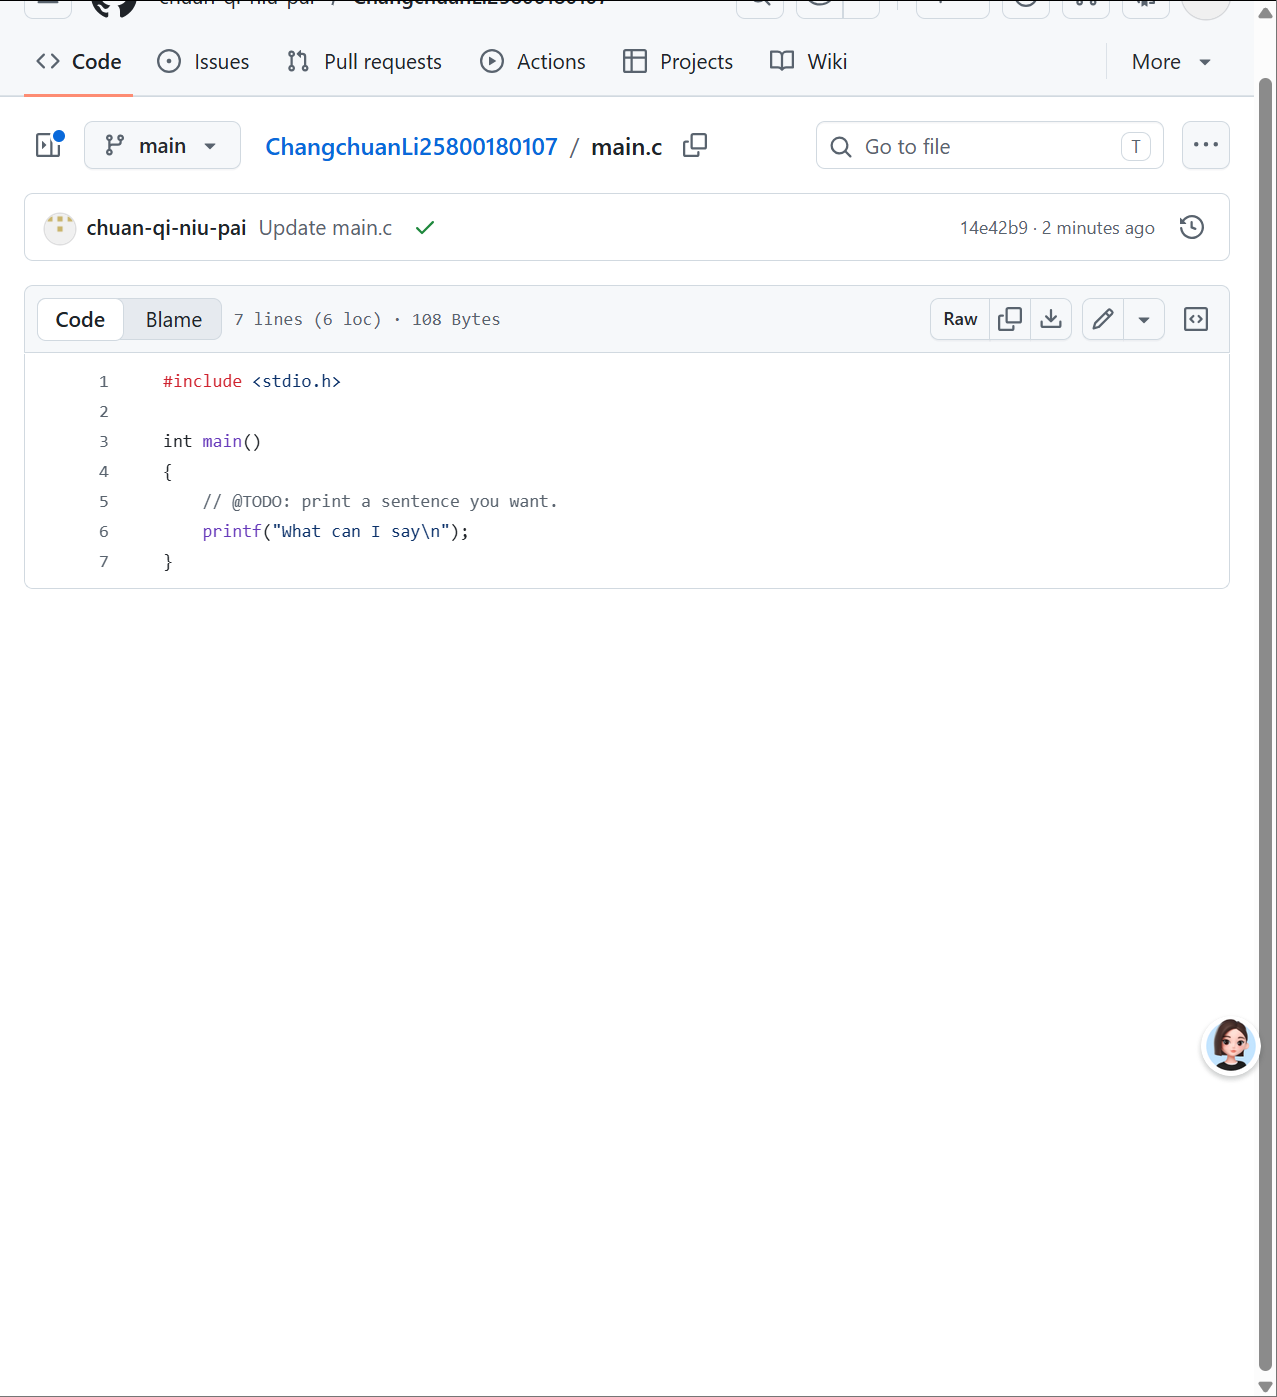
\includegraphics[width=0.85\textwidth]{images/main_c_github.png}
  \caption{GitHub 上 main.c 的内容}
\end{figure}

\section{任务 3：阅读概括与思考}

\par 我读了其中两篇：Conventional Commits（约定式提交）和 Semantic Versioning（语义化版本）。这两篇其实是配套的——前者管"每次提交怎么写"，后者管"版本号怎么升"，合在一起就是一套自动化发布的基础。

\textbf{Conventional Commits.} 它规定 commit message 写成
\begin{lstlisting}
<type>(<scope>): <subject>

[optional body]

[optional footer(s)]
\end{lstlisting}
的格式。\texttt{type} 用 \texttt{feat} 表示新功能、\texttt{fix} 表示修 bug、\texttt{docs} 改文档、\texttt{style} 调格式、\texttt{refactor} 重构、\texttt{test} 加测试、\texttt{chore} 搞构建或依赖；\texttt{scope} 可选，标注改动影响哪个模块；\texttt{subject} 用祈使句、一句话概括。正文和 footer 里可以写清楚"为什么这么改"，如果有不兼容的 API 改动，在 footer 里写 \texttt{BREAKING CHANGE:} 开头。

\par 这样做的直接好处是：别人扫一眼 \texttt{git log} 就知道这次提交干了什么，而不是看到一堆 \texttt{"update"}、\texttt{"fix bug"}、\texttt{"aaa"}。更重要的是工具能读懂它——比如 standard-version、release-please 这类工具会自动从 \texttt{feat:} 升 MINOR、从 \texttt{fix:} 升 PATCH、从 \texttt{BREAKING CHANGE} 升 MAJOR，自动生成 changelog 并打 tag，整个发版流程不需要人手写版本号。

\textbf{Semantic Versioning.} 它要求版本号必须是 \texttt{MAJOR.MINOR.PATCH} 三段：
\begin{itemize}
  \item \texttt{MAJOR}：做了不兼容的 API 修改时 +1，比如改了函数签名、删了接口；
  \item \texttt{MINOR}：以向下兼容的方式新增功能时 +1，比如多加了一个函数但旧用法还能用；
  \item \texttt{PATCH}：只做向下兼容的问题修复时 +1。
\end{itemize}
还约定了几个细节：0.x 初始开发阶段任何改动都可能不稳定，不承诺兼容性；预发布版本用 \texttt{1.0.0-alpha.1} 这种后缀；一旦发布就不能改内容，要改只能发新版本号。

\par 它解决的问题是"版本号到底代表什么"。以前看到 \texttt{2.4.1 -> 3.0.0} 心里没底，不知道要不要改自己的代码；现在一看就清楚：主版本号变了就要小心，次版本号变了可以放心升，修订号变了只是修 bug。npm、pip、cargo 这些包管理器也靠这个判断能不能自动升级，避免"升个小版本结果程序崩了"。

\textbf{为什么要学 Git.} 以前我对 Git 的理解停留在"改错了能退回去"，读完这两篇才意识到，Git 真正的价值不只是版本存档，而是一套人和人、人和机器之间的协作语言。commit message 规范、分支模型、语义化版本这些约定，让提交历史不只是硬盘上的快照，而是可读、可被自动化工具消费的工程记录——CI/CD、自动测试、自动发版、code review 全都建立在这个基础上。

\par 对个人来说最直观的感受是：分支让"试错"变便宜了。以前写代码我是不敢随便大改的，因为改坏了回不去；现在可以开一条 \texttt{feature/xxx} 分支随便折腾，搞砸了 \texttt{git switch main} 就回来了，main 永远是能跑的状态。这一学期后面几个 Lab 估计都要在 Linux 环境里写 C 代码，这种"随时能实验、随时能回退"的工作流应该会经常用到。

\section{任务 4：分支管理与冲突解决}

\textbf{操作步骤.}

\begin{enumerate}
  \item 确认在 main 分支、工作区干净：\texttt{git status}。
  \item 新建并切到 feature 分支：\texttt{git switch -c feature}。
  \item 在 feature 分支上把 main.c 第 6 行改成 \texttt{printf("Hello from feature branch\textbackslash n");}，提交：\\
  \texttt{git add main.c \&\& git commit -m "feat: change message on feature branch"}。
  \item 切回 main：\texttt{git switch main}，把同一行改成 \texttt{printf("Hello from main branch\textbackslash n");}，提交。
  \item \texttt{git merge feature}，因为两个分支都改了同一行，触发冲突。
  \item 手动编辑 main.c，删掉 \texttt{<<<<<<<} / \texttt{=======} / \texttt{>>>>>>>} 标记，保留 feature 分支的版本。
  \item \texttt{git add main.c \&\& git commit} 完成 merge commit，最后 \texttt{git push origin main} 和 \texttt{git push origin feature}。
\end{enumerate}

\textbf{冲突现场.} \texttt{git merge} 报 \texttt{CONFLICT (content): Merge conflict in main.c}，文件里出现冲突标记：

\begin{figure}[H]
  \centering
  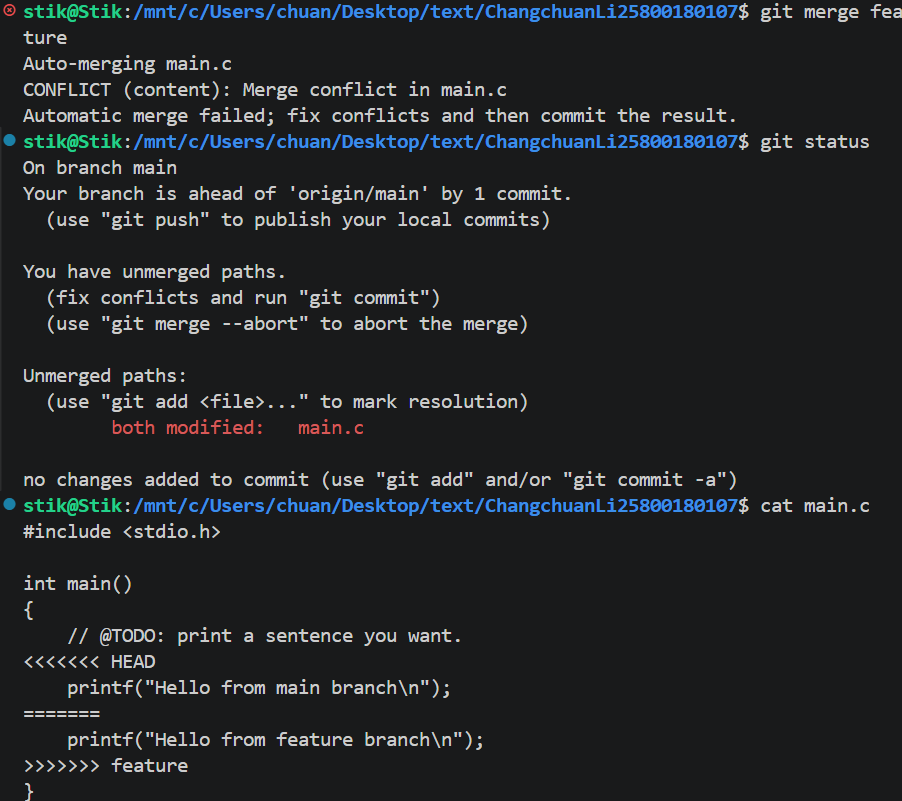
\includegraphics[width=0.9\textwidth]{images/terminal_conflict.png}
  \caption{终端报 CONFLICT，cat main.c 显示冲突标记}
\end{figure}

\begin{figure}[H]
  \centering
  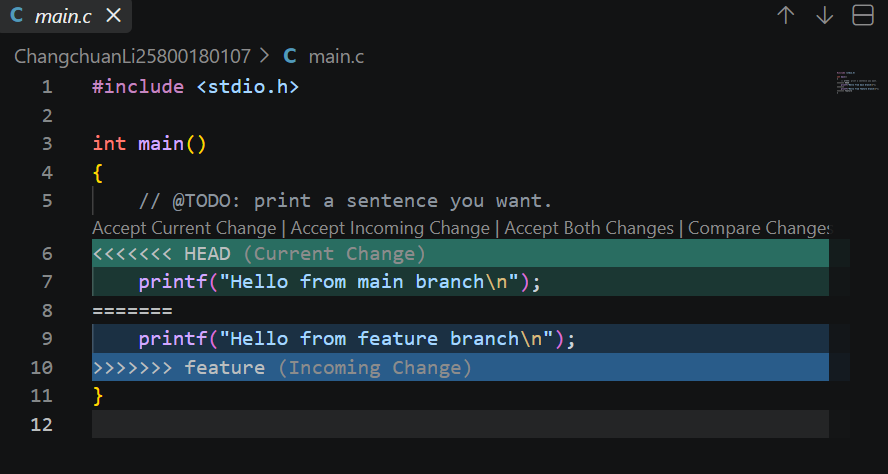
\includegraphics[width=0.8\textwidth]{images/vscode_conflict.png}
  \caption{VSCode 中的冲突视图（红绿块）}
\end{figure}

\textbf{解决冲突.} 删掉三对标记，保留 \texttt{printf("Hello from feature branch\textbackslash n");}：

\begin{figure}[H]
  \centering
  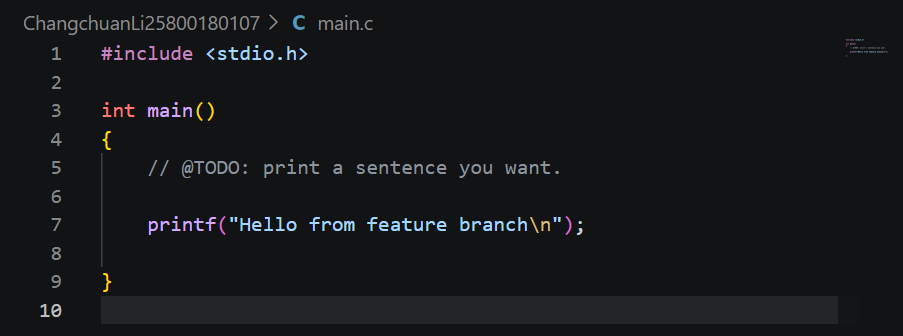
\includegraphics[width=0.7\textwidth]{images/resolved_main_c.png}
  \caption{解决冲突后的 main.c}
\end{figure}

\textbf{合并结果.} 本地 \texttt{git log --graph} 显示两条分支分叉再汇合：

\begin{figure}[H]
  \centering
  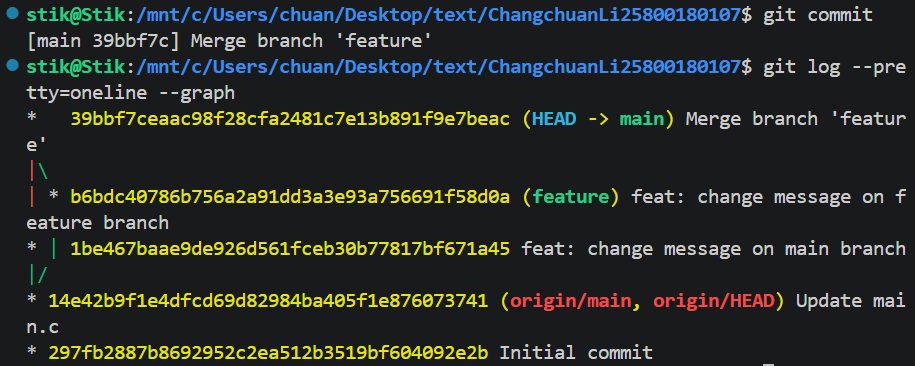
\includegraphics[width=0.9\textwidth]{images/git_log_graph.png}
  \caption{git log --graph 输出}
\end{figure}

推到 GitHub 后，Network 页面也能看到分叉合并的图形：

\begin{figure}[H]
  \centering
  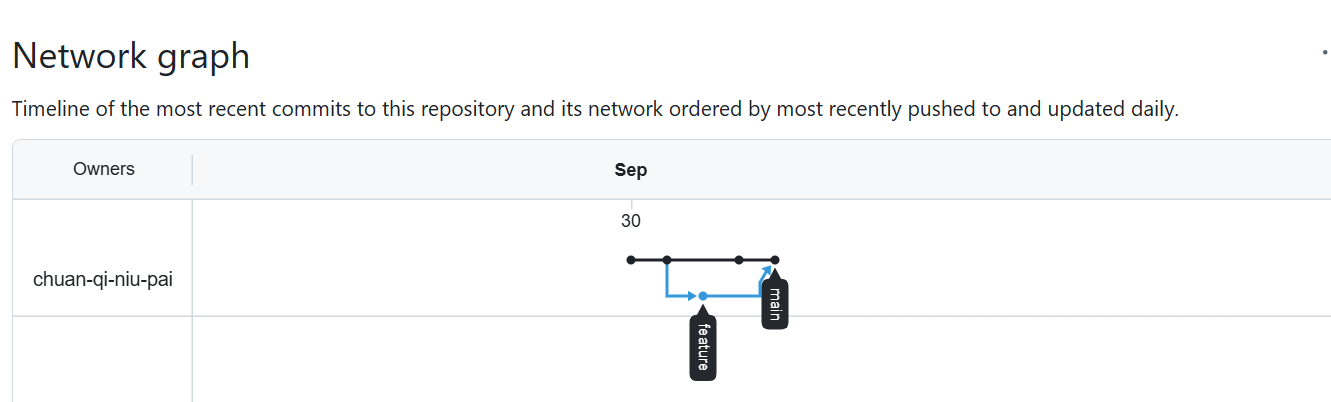
\includegraphics[width=0.9\textwidth]{images/network_graph.png}
  \caption{GitHub Network graph}
\end{figure}

\begin{figure}[H]
  \centering
  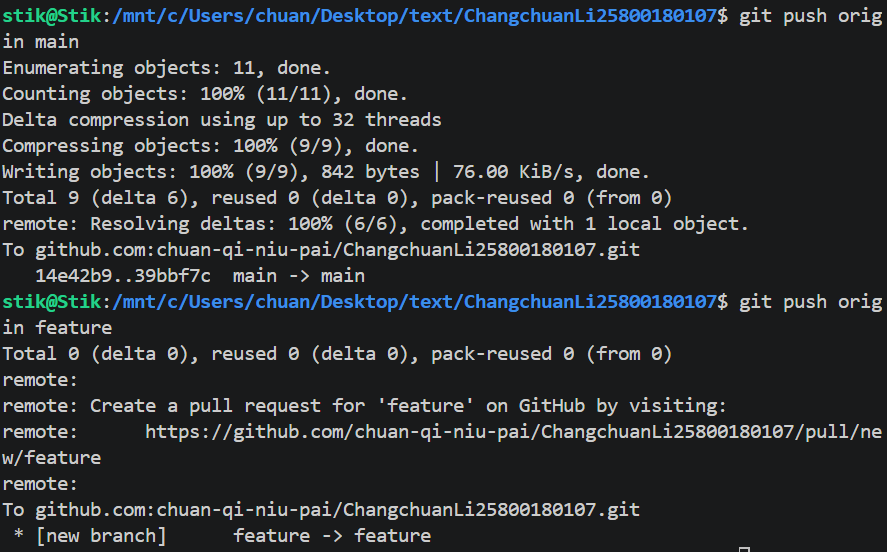
\includegraphics[width=0.9\textwidth]{images/push_output.png}
  \caption{push 到远程}
\end{figure}

\section{仓库链接}

\url{https://github.com/chuan-qi-niu-pai/ChangchuanLi25800180107}

\end{document}
